%%% Version 3.3 Generated 2016/11/10 %%%
%%% You will need to have the following packages installed: datetime, fmtcount, etoolbox, fcprefix, which are normally inlcuded in WinEdt. %%%
%%% In http://www.ctan.org/ you can find the packages and how to install them, if necessary. %%%
%%%  NB logo1.jpg is required in the path in order to correctly compile front page header %%%

\documentclass[utf8]{frontiersSCNS} % for Science, Engineering and Humanities and Social Sciences articles
%\documentclass[utf8]{frontiersHLTH} % for Health articles
%\documentclass[utf8]{frontiersFPHY} % for Physics and Applied Mathematics and Statistics articles

%\setcitestyle{square} % for Physics and Applied Mathematics and Statistics articles
\usepackage{url,hyperref,lineno,microtype,subcaption}
\usepackage[onehalfspacing]{setspace}
\usepackage{color, soul}
\usepackage{amsmath}
\usepackage{booktabs}
\usepackage{multirow}

\linenumbers
\newcommand{\FR}[1]{{\small \textcolor{red}{\hl{FR: #1}}}}

% Leave a blank line between paragraphs instead of using \\


\def\keyFont{\fontsize{8}{11}\helveticabold }
\def\firstAuthorLast{Sample {et~al.}} %use et al only if is more than 1 author
\def\Authors{First Author\,$^{1,*}$, Co-Author\,$^{2}$ and Co-Author\,$^{1,2}$}
% Affiliations should be keyed to the author's name with superscript numbers and be listed as follows: Laboratory, Institute, Department, Organization, City, State abbreviation (USA, Canada, Australia), and Country (without detailed address information such as city zip codes or street names).
% If one of the authors has a change of address, list the new address below the correspondence details using a superscript symbol and use the same symbol to indicate the author in the author list.
\def\Address{$^{1}$Laboratory X, Institute X, Department X, Organization X, City X , State XX (only USA, Canada and Australia), Country X \\
$^{2}$Laboratory X, Institute X, Department X, Organization X, City X , State XX (only USA, Canada and Australia), Country X  }
% The Corresponding Author should be marked with an asterisk
% Provide the exact contact address (this time including street name and city zip code) and email of the corresponding author
\def\corrAuthor{Corresponding Author} 

\def\corrEmail{email@uni.edu}




\begin{document}
\onecolumn
\firstpage{1}

\title[Running Title]{Predicting age with machine learning, using synchronized speech and MEG recordings in children} 

\author[\firstAuthorLast ]{\Authors} %This field will be automatically populated
\address{} %This field will be automatically populated
\correspondance{} %This field will be automatically populated
 
\extraAuth{}% If there are more than 1 corresponding author, comment this line and uncomment the next one.
%\extraAuth{corresponding Author2 \\ Laboratory X2, Institute X2, Department X2, Organization X2, Street X2, City X2 , State XX2 (only USA, Canada and Australia), Zip Code2, X2 Country X2, email2@uni2.edu}


\maketitle


\begin{abstract}

%%% Leave the Abstract empty if your article does not require one, please see the Summary Table for full details.
\section{}
For full guidelines regarding your manuscript please refer to \href{http://www.nontiersin.org/about/AuthorGuidelines}{Author Guidelines}.

As a primary goal, the abstract should render the general significance and conceptual advance of the work clearly accessible to a broad readership. References should not be cited in the abstract. Leave the Abstract empty if your article does not require one, please see \href{http://www.frontiersin.org/about/AuthorGuidelines#SummaryTable}{Summary Table} for details according to article type.

\begin{itemize}
\item Talk about dataset
\item Regression on age with multi-modal dataset + main result
\item Compare feature based classification + results and Augmented raw/real data +results
\item Should also specifically mention added a novel augmentation system
\end{itemize}


\tiny
 \keyFont{ \section{Keywords:} Deep Learning, Machine Learning, Convolutional Neural Networkds, MEG, Language Acquisition, Brain Computer Interface, Data Augmentation}
\end{abstract} 

\section{Introduction}

% Opening is pretty cliche

Machine learning (ML) has become an invaluable tool \cite{LeCun2015}. In computer vision, models such as those produced by \cite{He2015a} often perform difficult image recognition tasks with greater accuracy than human beings. In natural language, deep learning has become common for tasks like speech recognition \cite{Bahdanau}, comprehension \cite{Moritz}, and speech production \cite{VanDenOord}. ML has always been an important tool whenever a classification task presents itself in conjunction with complex data such as those recorded using MEG.

Various ML techniques have previously been used in a variety of fairly disparate tasks: detecting hand movement \cite{Asano2009}, identifying schizophrenia \cite{Ince2008}, and on discriminating between sets of imagined words \cite{Guimaraes2007}. To classify between three different hand movements\footnote{Corresponding to the signs in the game of `rock, paper, scissors'.}, \cite{Asano2009} used an adaptive spatial filter, principal components analysis (PCA), and a support vector machine (SVM) and achieved 62.6\% on held-out test data. Similarly, \cite{Ince2008} studied a single subject performing a working memory functional task while MEG data were recorded; an SVM with recursive feature elimination (SVM-RFE) was then used to both select a concise feature set and to identify schizophrenia. SVM-RFE recursively discarded features that did not significantly contribute to the margin of the SVM classifier to prevent excessive overfitting on the training set, and achieved 83.8\% to 91.9\% on the test data.

More similar to the data we consider presently would be work that focuses on \emph{speech generation} and ML, including \cite{Guimaraes2007}, who classified sets of 7-9 imagined words in two subtasks. In the first, the subject was simply required to attentively listen to a spoken word, while in the second the subject was shown each word visually and told to recite it silently. Those data were then examined using linear discriminant classification and SVM algorithms to classify each channel, and further analyzed in terms of the effects of spatial PCA, independent components analysis (ICA) and second-order blind identification decomposition. By combining channels, \cite{Guimaraes2007} achieved 60.1\% mean classification rate on nine auditory words and a 97.5\% maximum mean classification rate on two-word problems.

Previous work that heavily incorporates ML techniques is typically focused on brain-computer-interface (BCI) applications and takes a multi-stage approach to developing ML classifiers according to a \emph{feature based approach} (this is also applicable to similar data recorded via related means such as EEG ..). First, data are collected and pre-processed using a variety of techniques, such as cropping, trial averaging, normalization, band-pass filtering, and spatial transforms such as PCA, independent component analysis (ICA), common spatial patterns (CSP) \cite{Muller-Gerking1999}, and some more unique approaches like the xDAWN algorithm \cite{Rivet2009}. The goal of the preprocessing stage is to overcome the low signal-to-noise ratios typical of these types of recordings which complicate training. After these initial steps, features are calculated from these data, of which there are a plethora of successful options, but most commonly including spectral characteristics in the canonical activity bands ($\alpha$, $\beta$, ...) and statistical moments. Finally, these features and their associated class labels are used to train a classifier. Most commonly classifiers like support vector machines (SVM) or logistic regression are used as they are convex optimizations that are guaranteed to converge but surprisingly generalizability. An advantage of this approach is that expert knowledge about the data can help circumvent relatively poor signal quality and encourage ML models to distinguish between classes using established signal correlates. However, this comes with potential \emph{bias} of expert knowledge, and the underlying assumptions it may reinforce. In contrast, deep ML models (when they work) achieve many of the stages of this pipeline intrinsically, and so may reveal novel methods to pursue. Although these deep-learning architectures are fundamentally just arbitrarily flexible classifiers, when they are trained in an end-to-end fashion, their hierarchical structure also has the potential to perform signal-processing in early layers that may be informative when compared to more directed techniques.

Work specifically investigating end-to-end learning and deep-learning-like architectures with \emph{EEG} data has become more frequent recently; for instance, convolutional neural networks (CNN) have shown incremental improvements in BCI applications, and \cite{Schirrmeister2017} provided an informative comparison of many of these attempts. As a result of these works we notice a rough best-practices in architecture that has begun to develop that is not unlike the feature-based pipeline. Models that focus on different interconnections between successive layers of temporal convolution and spatial convolution operations perform the best in classification. Additionally, an early layer that performs some sort of spatial filtering (again mimicking the feature-based pipeline) has been used successfully by \cite{Lawhern2017}, \cite{Sun}, and \cite{Schirrmeister2017}. These early spatial filtering layers essentially disentangle the separate sources that are mixed at the cortical surface (and, in the case of EEG, have smeared due to other effects like the skull and scalp) \cite{ElectricFieldsOfTheBrain_ch5and6}. \cite{Schirrmeister2017} compared three models: a three-layer convolutional network in a configuration that simulates FBCSP, a five-layer deep convolutional network using the recently developed exponential linear unit (ELU) non-linearity \cite{Clevert} and residual networks \cite{He2015a}.

Each of these models was trained on the publicly available `BCI competition IV dataset 2a' and achieved results that surpassed the state-of-the-art with their first two models. These two successful models represented a good example of how a CNN that emulates a feature-based pipeline can successfully be trained from end-to-end. \cite{Lawhern2017} trained multiple CNNs, of equal parameter sizes, to classify four tasks with known characteristic signals, i.e., a P300 visual-evoked potential, error-related negativity, movement-related cortical potentials and sensory motor rhythm \footnote{This is the same dataset used by \cite{Schirrmeister2017} and as a benchmark in our work here.}. They compared the relative rank in performance of each model across all tasks to find the most generally appropriate architecture to train which they dubbed `EEGNet'. Each of their configurations employed a single early layer that performed spatial filtering, and compared models with two subsequent layers with an equal number of parameters, but differences in their span of temporal and spatial dimension. They found layers with receptive fields of $[2 \times 32]$ and $[8 \times 4]$, respectively, where the first dimension corresponded to a spatial dimension span and the second corresponded to a temporal one. Importantly, their optimal configuration employed two extremes of the parameter space they explored. The first kernel had the shortest length receptive field with respect to the spatial dimension, and the second had the shortest length with respect to the temporal dimension. This calls into question whether a more optimal solution may be found using even more narrowly focused receptive fields (e.g., single dimension convolutions).

\cite{Sun} used a CNN to predict the memory performance of their subjects. Their subjects were presented a set of spoken nouns, sequentially over headphones, to remember during an initial study session. They were then tested to indicate from 1 to 5 how much they felt they recognized words from a new set that included previously unheard words. They employed a three-layer CNN that, much like the other work above, began with a layer that develops a spatial filter (where their best performance is achieved with a single such filter), and then is followed by an exclusively temporal filter, and finally with a fully connected output layer before a final softmax output layer. They showed that their CNN outperformed a variety of other powerful techniques, including a continuous wavelet transform with an SVM and two fully-connected neural network configurations.

Others have begun to use recurrent neural networks (RNNs) \cite{Bashivan2016}, which are capable of much more complex processing since they are Turing-complete mechanisms. \cite{Bashivan2016} evaluated a mixed RNN and CNN architecture using EEG recordings of a working memory experiment, where subjects were asked to memorize a set of written characters and then indicate if a single presented character was in the original set. There, the EEG recordings were effectively translated into video streams, where each of the colours red, green, and blue corresponded to azimuthally projected (and then interpolated) images of three frequency bands. A pre-trained image-classifier CNN was used to extract a temporal stream of features and finally an LSTM network classified the sequence. Using this approach, the authors claimed to advance the state-of-art for this application from an error rate of $15.3\%$ to $8.9\%$.

These works typically focus on pushing their respective state-of-the-art classification accuracy against previous techniques. Few previous works examine the inner-workings of the models they develop, and fewer still consider investigating the model for insights into underlying neural activity that has taken place. The question of what a deep-learning architecture learns is an open and difficult problem, gaining much more research interest in the last few years. \cite{Schirrmeister2017} proposed a method of correlating convolutional filter outputs with activity in frequency bands of interest. Their method provides a good start for determining sensitivities to spectral content, but their approach requires strong assumptions where the spectral activity is focused. We consider an alternative approach that has shown some success in visualizing how CNNs trained with images perform the task of identifying which class an image belongs to \cite{Yosinski2015}. This approach generates artificial data that maximizes the activity of specific neurons through regularized optimization, to understand what data these neurons are ``looking for''. Of particular interest is when this is performed considering the output classes of a network, an ideal example. 

We present work that compares carefully selected deep-learning models trained end-to-end, against a feature-based approach, in their efficacy at classifying the age of children using MEG. We focus on a dataset of synchronized MEG and audio recordings of children performing speech elicitation tasks. We do this in an effort to develop models that are discriminative with respect to developmental differences in the different age groups. We first compare the predictive ability of the MEG and audio datasets using regression, then compare their powers to classify the age of the speakers with a variety of extracted signal features. Finally, we perform this classification again with an end-to-end classification approach that uses the raw data with negligible preprocessing, and we benchmark these models against previous state-of-art deep learning approaches for BCIs. Finally, we consider the efficacy of different data-augmentation strategies to help enable deep learning models that would otherwise require extremely large datasets. We contrast their efficacy at prediction and analyze the parameters the models develop. 


%% Old version that might still have some meat left on the bones.
% Juxtaposed to this specific domain knowledge approach is an \emph{end-to-end approach}. We define an end-to-end approach as training a ML model with raw data that has had minimal to no preprocessing applied to it all. Previous work in end-to-end training using brain signals and modern deep learning techniques have gained more attention in recent years and include: Schirrmeister {\em et al.} \cite{Schirrmeister2017}, who show an improvement over the previous state of the art in detecting hand and foot movement with their best models. They consider two layer convolutional networks in a configuration that simulates filter bank common spatial patterns (FBCSP) \cite{}, five layer deep convoluqtional networks and residual networks to classify movement on the publically available BCI competition IV dataset 2a \cite{}. Furthermore they employ a basic data augmentation technique of a sliding window cropping strategy that improves the performance of their models. We are unaware of any such work using MEG recordings. Another approach is \cite{Bashivan2016}... For more analysis that is particularly focused on CNNs, see \cite{Schirrmeister2017}. 


% Need to have some solid transition to the age/speech specific context before using any of the next points

% Talk about how we could select features by hand, based on previous work?

% For example, Doesburg {\em et al.} \cite{Doesburg2016} predict language ability as an increase in network synchrony with the increase of age during verb-generation (VG) tasks in children and adolescents. They observed a significant increase in the number of synchronous regions with older adolescents, compared with younger children. Furthermore, Yu {\em et al.} \cite{Yu2014} noticed distinct profiles of de-synchrony in VG tasks for children within five age ranges (i.e., 4-6, 7-9, 10-12, 13-15, and 16-18 years of age). These findings indicate the possibility of inferring a child's age from observed MEG data, provided the ability to convey synchronicity and coordinated activity.
% Previous work with electroencephalpgraphic (EEG) experiments use common spectral features such as the fast Fourier transform (FFT) magnitude and signal energy within consequetive time windows and various classifiers to accurately differentiating different persons \cite{Nguyen2012, Poulos2001}, and thus may represent synchronicity information. 

\section{Data}

\subsection{Primary dataset: Synchronized MEG and speech recordings}

These data were originally recorded to examine age- and sex-related developmental language differences in children by \cite{Doesburg2016} and \cite{Yu2014}. Table \ref{tab:subjects} summarizes some participant demographics. Each participant spoke English as their first language and had no known or suspected histories of speech, language, hearing, or developmental disorders, according to their parents. Prior to the experiment, children received two standardized clinical tests: the Peabody Picture Vocabulary Test (PPVT) \cite{Dunn97} and the Expressive Vocabulary Test (EVT) \cite{EVT}. All children's scores were at or above expected scores for their ages on the PPVT and EVT, and their speech showed neither signs of articulatory difficulties nor any significant effect of age, as visualized in Figure \ref{fig:ppvtevt}. In total, 80 participants were right-handed, 5 were left-handed, and 7 were ambidextrous, according to the Edinburgh assessment \cite{Oldfield}. %; there is no significant variation of handedness with age.

%% \begin{figure}
%% \includegraphics[width=\columnwidth]{PPVTEVT.pdf}
%% \caption{Normalized PPVT and EVT scores across ages for all participants. There are neither signs of speech production impairment nor effect of age on these assessments.}
%% \label{fig:ppvtevt}
%% \end{figure}

Three distinct speech-elicitation stimuli were used. The first two were of the monosyllable /{\em pah}/ and the multisyllabic sequence /{\em pah tah kah}/, respectively. These were simple enough for young children and are part of the diadochokinetic rate (DDK) test, which can be used to evaluate neuromuscular control in motor speech disorders. Prior to acquisition, the experimenter demonstrated the productions of each stimuli, without word-like prosodic patterns. The third experiment was an overt verb generation (VG) task in English, where subjects were presented with an image with which they were familiar, and were asked to produce a verb associated with the object \cite{Doesburg2016}.

Recordings were made in a sound-proof room, with each participant lying supine in a magnetically shielded room in the Neuromagnetic Lab of the Hospital for Sick Children in Toronto, using a CTF whole-head MEG system (MEG International Services Ltd., Coquitlam, BC, Canada). The system recorded all 151 MEG channels, and a single audio channel, with a sampling rate of 4 kHz.

Brief summary of some relevant age-related results from these works.

\subsection{Supplementary dataset: BCI Competition IV, Dataset 2a}

In an effort to compare the potential success of any end-to-end model developed to previous work, we also trained some of our end-to-end models using the BCI Competition IV EEG Dataset \cite{Tangermann2012}. This dataset has featured in several other attempts to apply deep learning and is freely available online \footnote{http://bnci-horizon-2020.eu/database/data-sets}.

These data consist of EEG recordings of 9 subjects performing 4 different imagined motor tasks: left hand, right hand, both feet, and tongue. These recordings were broken up into two separate sessions for each subject recorded on different days. Each of these sessions consisted of 6 sets of 48 trials separated by a short break, where the 48 trials were 12 executions of each of the 4 tasks. Thus a total of 288 trials were recorded per session. One session is considered training data, and the second is used as evaluation requiring some carry-over performance between days. The recordings consist of 22 EEG electrodes, and 3 monopolar EOG electrodes, all recorded at 250 Hz and bandpass filtered between 0.5 and 100 Hz. Additionally, a 50 Hz notch-filter was used to minimize line noise. The trials themselves are available as 6 second recordings, where the first two seconds consist of presenting each subject a fixation point. At 2s through 3.25s a task stimuli was presented to the subjects. There is additionally some EOG only trials per session that we discard. %\hl{this is probably a weakness of our approach as we might be learning some characteristic blinks, but we are basically comparing against other people who ignored this, not certain I like this...} \FR{It's ok. In the future, we could make use of it, or at least elegantly subtract it}

There are several challenges to using this dataset as a benchmark. It uses a different task entirely and contains EEG rather than MEG recordings, so there are far fewer EEG channels than the number of MEG channels from our primary dataset. The participants also come from a different population than the children and adolescents of our primary data. Regardless, we use this dataset to ensure that our model architectures have some sort of generalizability within this domain that can be compared against previous work. 

\section{Methods}

%Overview of experiments, data processing and analysis performed

\subsection{Data processing}

We resample MEG signals at 200 Hz, and band-pass filter between 0.5 Hz and 100 Hz, to remove offsets and accommodate the canonical ranges of $\delta$, $\theta$, $\alpha$, $\beta$, and $\gamma$ activity. Electro-ocular (EOG) artifacts are removed using automated blind source separation (Auto-BSS), and we measure signal complexities using fractal dimensions. Auto-BSS filters EOG artifacts using the SOBI algorithm described in \cite{eog}. This preprocessing step is common to both our feature-based and end-to end approaches.

To further preprocess our data, for our feature-based approach, we apply info-max independent component analysis (ICA) \cite{Bell1995} to determine statistically independent sub-components of the MEG recordings, across all subjects. This is done by appending MEG recordings for all subjects into a single 151-channel matrix for each of the 3 speech-elicitations: /{\em pah}/, /{\em pah tah kah}/, and the VG task. We then apply the resulting sphering and weight matrices, determined by ICA for each test condition, to each subject's respective recordings. These recordings (i.e., both MEG and audio separately) are then separated into windowed epochs corresponding to frames $-500$ ms to $+1500$ ms around the onset of the stimuli prompt.

\subsection{Feature extraction}

We extract 156 acoustic features and 4681 MEG features from each epoch using openSMILE \cite{Eyben13-RDI}. These are calculated using 50 ms rectangular windows, with a 25 ms overlap resulting in 79 windows per datapoint.

\subsubsection{Audio features}

Features to represent spectral activity are calculated, for each window, using both a 128-point fast Fourier transform and linear predictive coding coefficients. Additionally, the statistical moments: mean (also absolute mean, quadratic mean, and aforementioned means calculated using only non-zero values), variance, skewness and kurtosis are calculated. Finally, the root-mean-squared and log of the signal energy are also calculated for each window.

\subsubsection{MEG features}

We extract 31 features for each of the 151 independent components derived from the MEG data. These consist of an 8-point fast Fourier transform, statistical moments, and energy calculation identical to the audio signal, and the autocorrelation function (ACF) calculated using the fast Fourier transform (FFT) and its inverse (iFFT) for window $w$:

% Probably could use some more discussion of the features here?

\begin{equation}
  ACF(w) = iFFT(|FFT(w)|^2)
  \label{eq1}
\end{equation}

\subsection{Sensor projection}\label{sec:sens_proj}

To better represent the spatial structure of the recordings, we experiment using a series of image representations of the data. The data are originally represented as 2-dimensional arrays whose first dimension corresponds to samples in time, and the second dimension is of length 151 corresponding to the 151 MEG channels in no spatially significant ordering. To represent the spatial nature of the data, the locations of the 151 channels of the MEG sensor array for each experiment are projected using an azimuthal projection (also known as polar projection) onto a two-dimensional grid sized $h \times v$, and then the raw values of each sensor are  interpolated based on the nearest (projected) sensor across this grid to generate a series of images, i.e. a three dimensional datapoint with dimensions $samples \times  h \times v$ where $h$ and $v$ are hyperparameters that can be selected. A similar approach was used in \cite{Bashivan2016}, where EEG data was projected and then interpolated into a series of images, but instead of using raw data as we do here, they created multiple channels which represented different spectral features (in their case the $\theta$, $\alpha$, and $\beta$ frequency bands). We choose not to take this approach, as this would increase the dimensionality of the problem immensely and, as implemented by \cite{Bashivan2016}, the approach requires a strong assumption of how distinguishing data distributes across particular spectral bands.

\subsection{Data augmentation}

To facilitate end-to-end learning, we employ two techniques that produce multiple usable training points from the same recordings as described below. 

\subsubsection{Cropping}

Here, the entire trial is split into multiple training examples by taking subsections of each trial that still include the event onset. Effectively, rather than one training datapoint for each trial, a sliding window smaller than the length of the trial is used to crop many points, where each point has the event onset localized in a different place. The premise behind this augmentation is that with the event localized in different places, an architecture like a convolutional or recurrent network can learn temporal filters that are agnostic of a specific onset time and thus should be more generalizable. Previous work that has taken this approach include \cite{Schirrmeister2017, Sun}. %We uniformly select a single crop position for each trial every epoch, rather than inflating the number of points in the dataset.

%% \subsubsection{Subsampling}

%% We take advantage of the high sampling rate of the recordings ($4kHz$) being used with respect to the frequency ranges that that we keep  for analysis and examine whether different sub-sampling of the data is a viable augmentation strategy. Filtering is still applied as before to minimize aliasing artifacts, and then we augment the number of samples by re-sampling at a frequency of $200 Hz$

\subsubsection{Noisy sensors}

To our knowledge, there are few examples of data augmentation with respect to the location of channels for training neural networks. In \cite{Krell2017}, the authors developed a rotational strategy of EEG data augmentation where they saw success in increasing classification accuracy for their particular processing chain using rotations in three-dimensional space of $\pm 18^{\circ}$ around the y- and z-axes. We consider an alternative augmentation strategy that we hypothesize may be more appropriate for MEG data, where the location of a sensor (after projection \ref{sec:sens_proj}) is subject to Gaussian distributed noise (truncated within a single deviation), with the recorded position being the mean of the distribution and variance being a hyperparameter to be selected. As MEG helmets tend to be slightly large for most people, and this effect is exagerated when considering small children such as in our primary dataset, this noisy sensor augmentation is a simple modeling of this source of error to enable better generalization with this higher dimensional (sensor projection of course increases the dimensionality of the data significantly) data. \hl{We need to ask LP (or does FR know the answer to this?) if this is already accounted for somehow, in particular if there is some set of adjustable sensors I might be unaware of}

\subsection{Data analysis}

First, we identify correlations among extracted features, in order to demonstrate evidence for predictive potential. We then train regularized multilinear regression models to predict a subject's age.

All regression and classification models are evaluated using the same held-out test subjects, using five-fold cross-validation. The test set has a nearly identical distribution of age.

\subsubsection{Correlation}

We use standard Pearson correlation between the extracted MEG and audio features, for each experiment set separately. We set significance for $p$-values at $\alpha = 10^{-4}$ and consider correlated featires asthose with absolute value $\text{abs}(r) > 0.2$. For each experiment, we then examine the independent component that had the highest correlations of its features with respect to audio features, to determine if there were any noticeably consistent brain locations that were being emphasized. These are plotted in Figure \ref{fig:components}. Furthermore, we compute correlation of MEG and audio features, with respect to age, over the entire data set, to identify features with a potentially stronger predictive capability for regression.

\subsection{Training procedure} \label{sec:train_proc}

Each model is tested using 5-fold cross-validation against a held-out group of subjects. The test subjects are selected to have a similar distribution of the number of trials in each age range, and closely match the standard deviation of age between all subjects. The remaining subjects are ordered based on the number of trials they performed and distributed across the 5 folds in this order. In the supplemental dataset, the training versus test datasets are separated in advance for intra-subject training.

We use Keras \footnote{https://keras.io/} with a Tensorflow \footnote{https://www.tensorflow.org/} backend to build all of the following models, and use either stochastic gradient descent or the Adam optimizer  when performing back-propagation updates. When training the neural networks, we select between three different activation functions: the rectified linear unit (ReLU) \cite{He2015a}, the exponential linear unit (ELU) \cite{Clevert}, and the scaled ELU (SELU) \cite{NIPS2017_6698}. All layers are batch-normalized \cite{Szegedy2015} after activation, with dropout and optional pooling. We additionally employ L2-norm weight regularization for all trainable weights, excluding those of RNNs and dropout \cite{} after all fully-connected layers, and spatial dropout \cite{} to all convolutional layers. These techniques were not necessarily applied to the FBCSP-like model from \cite{Schirrmeister2017}, which we reproduced by examining their source code.

All hyperparameter selection is done using Bayesian parameter optimization with Hyperopt \cite{Bergstra2013}  including: learning rate, regularization penalty, dropout rates, number of adjacent activations to pool, number and layers of hidden units, receptive fields, and activation functions for all appropriate models. \hl{Should we put an appendix that describes the parameter space and some of the selected parameter models? Maybe at the very least have explicit parameters for best few models to facilitate any reproduction.}\FR{Yes, if it's not too much trouble}

\section{Neural network architectures}

\subsection{Fully-connected feed-forward neural network}

This consists of 1-3 layers (a hyperparameter we search for) of neurons, fully connected by weights that are trained using the ubiquitous back-propagation method \cite{Lecunn_phd, GoodfellowTextbook} and gradient descent (in addition to other optimization techniques like \cite{adam, rmsprop, etc}). Crucially, the output of each neuron has a non-linear operation (in our case we select among three, seen in Section \ref{sec:train_proc}) applied to the weighted sum of all incoming connections. %This applies for the most part all neural network implementations, and allows them to learn arbitrary functions that separate output labels.

\subsection{Convolutional neural network}

% Figure for all the remaining architectures would be best.

A convolutional neural network (CNN) \cite{LecunnMNIST, GoodfellowTextbook} is a variation on the feed-forward neural network that shares incoming weights that are swept like a convolution operation over input tensors. This is done to reduce the number of parameters and, as a result of the convolution structure, develop translation-invariant features. This can be juxtaposed against the feed-forward network's operations that are more akin to mask-like operations that are compounded into an arbitrary function. A CNN is said to have layers with a \em{receptive-field} or to have a \em{kernel}, this refers to the number of shared weights (or equivalently, the number of inputs used at each convolution). This kernel takes some {\em stride}, which refers to the number of inputs in the datapoint to proceed ahead before performing another operation. The number of different kernels (or filters) refers to the number of independent sets of weights learned for each layer (where each filter for the most part has the same receptive field and stride). It is common to apply pooling layers \cite{} after convolutional layers to encourage differentiation between filters and translational in-variance of filters, so we apply max-pooling \cite{} layers after all convolutions unless otherwise noted.

\subsubsection{ShallowFBCSP CNN}

This is a CNN architecture used by \cite{Schirrmeister2017} that uses unconventional (for a convolutional network) activations and connections to emulate a \emph{filter-bank common spatial pattern} model (FBCSP) \cite{KaiKengAng2008}. Despite employing a CNN-like architecture, there is a lack of convolution operations across the channels themselves (this is also evident in \cite{Lawhern2017} and \cite{Sun}), as the receptive field spans the entire set of channels. Also, in an effort to stay true to the CSP spatial filter that this layer emulates, \cite{Schirrmeister2017} elected that this layer should have no non-linear operation applied to its outputs. Although this may encourage the model to behave more like the FBCSP algorithm, it neglects a typically crucial step for neural network models.

\subsubsection{Spatial summary CNN} \label{sec:scnn}

This architecture is inspired by the success of non-neural network pre-processing that use spatial filters to transform data before any classifier is used, such as the \emph{ShallowFBCSP}. Here, the spatial convolutions ultimately span the length of the incoming channels, but rather than being a single linear layer we introduce non-linearity and multiple convolution layers that work together to construct a more flexible spatial filter, but still one that is constrained by the sharing of weights. We select a hyperparameter indicating the depth of the spatial filter, and then stack convolutional layers, where each layer reduces the spatial dimension until the final layer completely collapses it to 1. After this, a number of temporal filters (i.e., convolutions over the temporal dimension) are applied to the new spatial mapping (the number is also a selected hyperparameter), and an optional average pooling layer to reduce the number of parameters and effectively low-pass filter these new features.

The CNN can be seen as a mapping from $R^{T \times C \times 1}$ to $R^{T \times 1 \times S}$ (the spatial filtering) to $R^{T' \times 1 \times F }$ (the temporal filtering) where $T' \leq T$, $C$ is the number of recording channels, $S$ is the number of spatial transformations, and $F$ is the number of temporal filters. In other words a set $S$ of non-linear spatial transformations are applied to the $C$ channels, and then a set of $F$ temporal filters are applied to these new sequences. 

\subsubsection{Short field 2D convolutions}

This architecture extends the spatial summary CNN to data that are represented as 2D interpolated images, rather than vectors of channel values. The difference here is that 2D convolutions make up the spatial mapping rather than single dimensional ones.
 
\subsection{Recurrent neural networks} \label{sec:rnns}

Recurrent neural networks (RNNs) are different from the previously discussed architectures, as RNNs feed their outputs or hidden layers back to their inputs as they process incoming data. In this way, and to varying extents, the output of the network at some point $output_t$ is dependent on the output of the network up to that point $output_0, output_1, ..., output_{t-1}$ and by extension also dependent on the sequence of inputs that produced each output. 

The long short-term memory (LSTM) \cite{Hochreiter1997a} recurrent network cell circumvents a critical challenge in using back-propagation with RNNs by adapting their recurrent connections with back-propagation {\em through time}. In short, a problem arises where gradient values from the end of the sequence can very easily become too large or too small as it is propagated back through the network and is positively enforced. LSTMs introduce at least three \emph{gated} cells which preserve values until they are required  \cite{GravesRNNBook}.

Our implementation uses bi-directional LSTMs (optionally with an attention mechanism as described below) \cite{GravesRNNBook}. This is a slight modification where two stacked LSTM networks are trained, one in the forward direction through the data sequence and a second is trained backwards. The data from both is typically combined through a concatenation of output vectors or summation of outputs (here, we concatenate the outputs). We select whether to use the full LSTM output sequence, or exclusively the last state output as part of our hyperparameter search. Using the final outputs of a sequence tends to be good practice for classification \cite{}, but we still consider the output of the entire sequence, as the variability introduced via the cropping mechanisms might be aided by this \FR{how?}. Additionally, in our preliminary experiments, we see surprisingly few indicators of overfitting due to over-parameterization, as typically the observed validation curves reach their minimum and begin to deteriorate well before models strongly fit to the training data. 

\subsubsection{Attention}

% Definitely want figure for this section

Attention mechanisms have been applied to information retrieval \cite{Moritz}, machine translation \cite{machine_translation}, and speech recognition \cite{Bahdanau}. They are also regularly employed in transduction tasks like image captioning \cite{XuKELVINXU, etc.} and visual question answering \cite{}. The general principle remains mostly the same across all of these implementations, i.e., to focus a network's current machinations over a sequence of features by relatively weighting each feature over the entire sequence given the current scenario. The formulation that tends to be easiest to integrate is a `soft-attention' model \cite{XuKELVINXU}, as it is trained along with the rest of the model using back-propagation. Considering a sequence of features to which we would like to attend, denoted here as $\{f_0, ..., f_{T-1}\}$, and a sequence of current states $H = \{h_0,...,h_{T-1}\}$, we calculate \emph{soft-attention} $\alpha_t$: 

\begin{equation} \label{eq:attn_nrg}
  e_{t} = a(f_{t}, H) , \alpha_t =  \frac{\exp(x_{t})}{\sum_{j=0}^{T-1}exp(x_{j})}
\end{equation}

Where $a()$ is an arbitrary function\footnote{We use a multi-layer network similar to the original formulation in \cite{XuKELVINXU}, but the number of layers used is a hyperparameter determined during search, and units per layer equal to the number of hidden units with the associated LSTM.}, and the \emph{softmax} function is applied along the sequence axis. This soft attention is then used as the weights of a weighted sum of the feature sequence to produce a new feature sequence for all features $j$: 

\begin{equation} \label{eq:attn}
    f_{tj}' = \sum_{i=0}^{T-1} f_{ij} \alpha_{ij}
  \end{equation}

In our experiments, we employ an architecture that is very similar to the encoding stage employed in \cite{Zhu} for the purpose of image-directed question answering. Those authors used a pre-trained CNN and an LSTM-based encoder that was fed attention weighted inputs. The attention mechanism provided an average weighting of the different convolutional feature maps which were combined with one-hot encoded word vectors representing the words in the questions.


In contrast, our implementation does not use a pre-trained CNN, but trains convolutional layers at the same time as the rest of the model. The attention serves as a mechanism to fuse the spatial summary architecture and the LSTM architectures together. The attention provides an average weighting of the features after spatial mapping and filtering (described in Section \ref{sec:scnn}) over time.

\subsection{Model analysis and visualizations}

Explaining \em{what} a trained neural network has learned is an on-going area of research, and a particularly important one. For neural-network based models to be significantly useful beyond their successes as classifier tools, understanding what they are doing is crucial. There are currently two directions of work that address this, one in which (optionally modified) selections from datasets are fed into an already trained model and the sensitivity of specific layers or neurons are examined, and a second in which artificial data is developed by maximizing the outputs of a trained model with respect to artificial data (with no reliance on training points in particular) \cite{Yosinski2015}. We take the latter approach to develop artificial inputs that \em{maximally activate} key points in our models. This involves performing regularized gradient-ascent of an output $f_o$ within the fully trained model with respect to the input $x$. So that we produce an artificial datapoint $x_{max}$ where:

\begin{equation} \label{eq:max_act}
  x_{max} = arg_xmax(f_o - R(x))
\end{equation}

Here we summarize any regularization penalties as $R(x)$. \cite{Yosinski2015} show that crucial to the success of this technique is to ensure good prior distributions on the artificial data, so in this spirit we begin with randomly initialized data that has a spectral density that decreases with $1/f$ and zero mean, thus conforming conforms to general encephalographic recordings. We also use L2 regularization on our data-points which helps prevent unbounded growth during the ascent which in effect prevents some strongly relevant features from eclipsings some features that are important but less impactful on the outputs. The update rule is then:

\begin{equation} \label{eq:max_act_update}
  x \leftarrow \eta \big(x + \frac{\partial }{\partial x}(f_o - \theta \cdot {}\sum_ix_i^2) \big)
\end{equation}

Where we heuristically selected a step increase of $\eta = 0.2$ and L2 penalization of $\theta = 0.05$. We then iterated up to 10000 times, stopping if no progress was made for more than 5 steps. Additionally we normalized the derivative in eq. \ref{eq:max_act_update} for each step by it's RMS value to make more stable (less oscillatory) progressions.

We construct maximal inputs for two sets of input-output pairs in the trained (primary dataset) end-to-end models. The first is between the model's normal input, and the end of the final-most spatial convolution layers. This is to construct a set of spatial filters that can be examined much like our ICA spatial filters. The second input-output pair is between the input to the first temporal convolution (the output of the last spatial) and the final model output (classification stage). This is to generate data that highlights temporal features of the patterns of mixed senors, which we do by performing calculating a spectrogram for each component and output class.

\section{Results}

\subsection{MEG vs. audio features}

Only $0.0163$\%, $0.0116$\% and $0.132$\% of the $156 \times 4681$ correlations using the /{\em pah}/, /{\em pah tah kah}/ and verb-generation data respectively are significant (after consideration of our defined thresholds). This suggests little redundancy between the MEG and audio features analyzed and supports the consideration of a combined prediction model and a much more complex connection between phenomena. Of these significant correlations, three audio features stand out as more strongly correlated to MEG data. These features correspond to sequential FFT bins that represent the frequency range 340-400 Hz. In therms of strongly correlated MEG features: the autocorrelation measure (eq. \ref{eq1}) is the most intensely correlated MEG feature across and is so across three independent components common to all three experiments.

\begin{figure}[t]
  \centering
  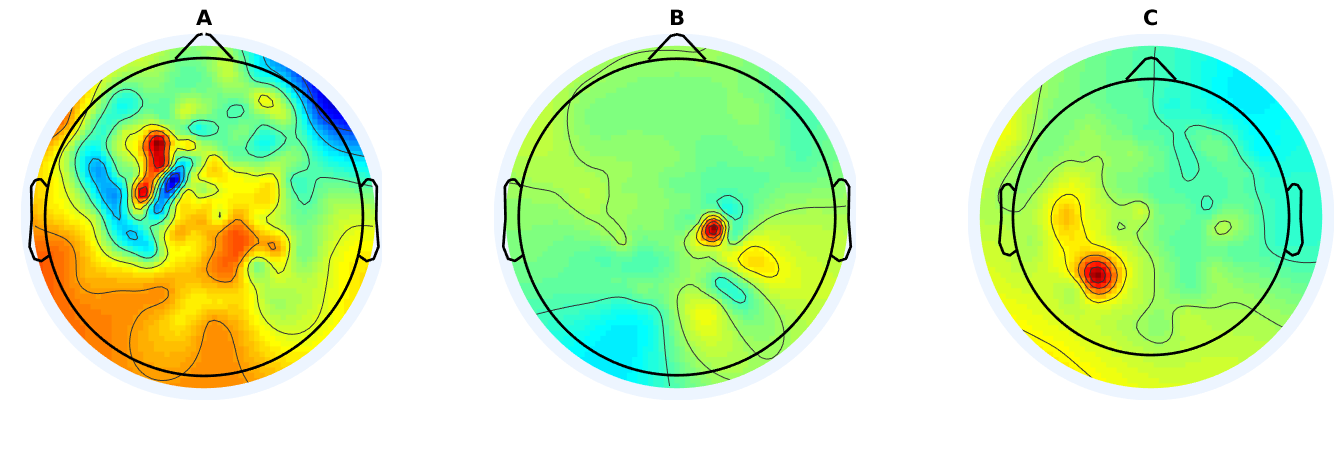
\includegraphics[width=\linewidth]{AllComponents.png}
  \caption{Graphical illustrations (using \cite{Delorme04eeglab}) of the independent components with features most correlated with audio features, from left to right, /{\em pah}/, /{\em pah tah kah}/ and verb generation experiments. These are generated using the ICA weight matrix interpolated over MEG sensor locations. The component depicted in A hints at significant activity localized near Broca's area, and the component in C is more localized in Wernicke's area. These localizations seem appropriate for the tasks. Component B on the other hand is not so conveniently suggestive of classical language regions.}
  \label{fig:components}
\end{figure}
 
\subsubsection{All features vs. age}

When correlating with age, 172 features have significant values, all of which are MEG features. This includes the autocorrelation features of eight ICA components (including the first (highest entropy) component) in addition to the entire available frequency spectrum of four of these components. \hl{TODO: Re-visit these for what f-ranges they correspond to}.

The correlation of a single ICA component has correlation coefficients $\text{abs}(r)>0.3$ for nearly all of its features, which is true of no other components considered. \hl{TODO: image of this component} Three other components also have features with correlation $\text{abs}(r)>0.3$, for features that corresponded to various mean variants.

\subsection{Regression}

\begin{table}[t]
  \centering
  \label{tab:reg_results}
  \begin{tabular}{ l | c | c | c | c }
    \toprule
    \textbf{Feature set} & \textbf{RMSE Mean} & \textbf{RMSE Deviation} & \textbf{MAE Mean} & \textbf{MAE Deviation}       \\
    \toprule
        Audio~~~                             & ~~~$4.59$         &     $0.45$     & ~~~$3.34$         &     $0.37$       \\
        MEG~~~                               & ~~~$19.0$         &     $16.5$     & ~~~$9.96$         &     $7.86$       \\
        Audio+MEG~~~                         & ~~~$63.7$         &     $61.0$     & ~~~$63.7$         &     $61.0$       \\

        \midrule
       
        MEG (red.)~~~                        & ~~~$5.51$         &     $2.12$    & ~~~$3.28$          &     $0.30$       \\
        Audio+MEG (red.)~~~                  & ~~~\textbf{2.97}  &     $2.05$    & ~~~\textbf{2.97}         &     $2.05$      \\

    \hline
  \end{tabular}
  \caption{Root mean squared error (RMSE) and mean absolute error (MAE), in years, of 5-fold cross validation for each of the feature sets. Audio features combined with reduced MEG features show the best prediction capability. Bold indicates the best RMSE.}
\end{table}

Regressions across the 5 folds suggest that a multilinear regression model trained using both audio and the reduced (i.e., highly correlated) MEG feature sets performs better than either audio or MEG feature sets alone. Without reducing the MEG feature set, regression performance is quite poor. Table \ref{tab:reg_results} shows the means and variances of root mean squared error (RMSE) and mean absolute error (MAE) values on regression, given various combinations of feature sets. There appears to be a marked decrease in error when combining audio features with a reduced set of MEG features result in the best accuracy on average.


% FR: in future, a measure of mutual information should be computed.

\subsection{Feature-based classification}

\begin{table}[t]
  \centering
  \label{tab:feat_results}
  \begin{tabular}{l l | c | c}
    \toprule
    \textbf{Dataset} & \textbf{Model} & \textbf{Mean \%} & \textbf{STD. \%} \\
    \toprule
    \multirow{3}{*}{Audio}
                     & Logistic Regression & 17.5 & 4.42  \\
                     & Linear SVM          & 17.2 & 5.15  \\
                     & Shallow NN          & 18.9 & 6.00  \\
                     & LSTM + Attention    & 23.8 & 7.08  \\
                     & SCNN                & 15.6 & 4.00  \\
    \midrule
    \multirow{3}{*}{MEG}
                     & Logistic Regression & 16.5 & 6.84  \\
                     & Linear SVM          & 19.2 & 6.07  \\
                     & Shallow NN          & 27.1 & 0.80  \\
                     & LSTM + Attention    & 26.0 & 0.80  \\
                     & SCNN                & 24.8 & 8.78  \\

    \midrule
    \multirow{3}{*}{MEG reduced.}
                     & Logistic Regression & 27.9 & 2.52  \\
                     & Linear SVM          & 28.5 & 0.79  \\
                     & Shallow NN          & 28.1 & 5.91  \\
                     & LSTM + Attention    & 20.7 & 6.90  \\
                     & SCNN                & 22.4 & 4.96  \\
    \bottomrule
  \end{tabular}
  \caption{Classification accuracy mean and standard deviation using one of three datasets, and three different basic classifier models. \FR{there are a lot of NaNs here... what is the cause? Should we reduce the number of covariates, e.g? We don't want this}}
\end{table}

% I don't think much space should be devoted to the analysis of the parameters of these models

\subsection{End-to-end classification}

\subsubsection{Primary dataset}

\begin{table}[t]
  \centering
  \label{tab:end2end_results}
  \begin{tabular}{l l | c | c}
    \toprule
    \textbf{Feature set} & \textbf{Model} & \textbf{Mean \%} & \textbf{Variance \%} \\
    \toprule
    \multirow{3}{*}{Raw Data}
                         & LSTM + Attention    & 28.1 & 5.00  \\ 
                         & SCNN                & 28.6 & 7.91  \\
    \midrule
    \multirow{3}{*}{Temporal Augmentation}
                         & LSTM + Attention    & 26.3 & 2.07  \\ 
                         & SCNN                & 32.4 & 10.9  \\
    \midrule
    \multirow{3}{*}{Spatial Projection}
                         & SCNN                & 21.9 & 2.20  \\
    \midrule
    \multirow{3}{*}{Spatial Augmentation}
                         & SCNN                & 15.0 & 5.10  \\
    
    \bottomrule
  \end{tabular}
  \caption{Classification accuracy across the seven age categories, using minimally pre-processed data input under different augmentation strategies and models. We do not combine spatial and temporal augmentation as they should provide additive gains \hl{but realistically its because the spatial augmentation models take a long time to train.}}
\end{table}



\subsubsection{Secondary dataset}

\begin{table}[t]
  \centering
  \label{tab:end2end_results}
  \begin{tabular}{l l | c | c}
    \toprule
    \textbf{Feature set} & \textbf{Model} & \textbf{Mean \%} & \textbf{Variance \%} \\
    \toprule
    \multirow{3}{*}{No Augmentation}
                         & FBCSP-CNN           & 70.9 & 12.6  \\
                         & SCNN                & 72.6 & 10.7  \\
                         & LSTM + Attention    & \textbf{73.3} & 13.6  \\ 
    \midrule
    \multirow{3}{*}{Temporal Augmentation}
                         & FBCSP-CNN           & 65.6 & 12.2  \\
                         & SCNN                & 35.1 & 14.2  \\
                         & LSTM + Attention    & \textbf{66.6} & 17.1  \\ 
    \bottomrule
  \end{tabular}
  \caption{Classification accuracy of SCNN and LSTM with attention models proposed in this work as compared to the convolutional FBCSP from \cite{Schirrmeister2017}. Despite some marginal increases accuracy, none of these are significant increases, as they substantially fail to meet p < 0.05 in a Wilcoxon signed rank test (each new model compared against FBCSP-CNN).}
\end{table}

Here we verify that the SCNN and LSTM + attention models are general enough to apply to a different application and achieve results that are comparable to the state-of-the-art. The accuracy improvements seen here with respect to the convolutional FBCSP are not statistically significant, SPECIFIC QUANTITY NEEDED -- Kruskal Wallis all examples ignoring the SCNN outlier, and determine if all part of the same group. If we consider the fact that these models have nearly two orders of magnitude more parameters, it is clear that they are not as parameter efficient. Here we see further evidence that the temporal augmentation strategy for these models does not provide an increase in performance for the models we have selected, as the SCNN model with a temporal augmentation strategy seems to underperform by a large margin in comparison to it's un-augmented counterpart (under a Wilcoxon Signed Rank test...).

\subsection{Model Analysis}

\begin{table}[t]
  \centering
  \label{tab:end2end_results}
  \begin{tabular}{l l | c | c}
    \toprule
    \textbf{Feature set} & \textbf{Model} & \textbf{Mean \%} & \textbf{Variance \%} \\
    \toprule
    \multirow{3}{*}{MEG reduced.}
                         & Logistic Regression    & 63.5 & 5.64  \\ 
                         & Shallow NN             & 69.2 & 5.74  \\
    \midrule
    \multirow{3}{*}{Raw Data}
                         & LSTM + Attention    & 92.6 & 5.79  \\ 
                         & SCNN                & 95.1 & 2.31  \\
    \midrule
    \multirow{3}{*}{Temporal Augmentation}
                         & LSTM + Attention    & NaN & NaN  \\ 
                         & SCNN                & 89.2 & 7.93  \\
    
    \bottomrule
  \end{tabular}
  \caption{Classification accuracy when constrained to the binary classification problem of $age  >=  10$ versus $age < 10$.}
\end{table}

Here we notice what appears to be a startling difference in performance between feature and end-to-end approaches.

Kruskal Wallis 

\section{Discussion}

%% Taken from IS paper, still needs to be changed

This work combines and compares aligned audio and MEG data, in a few speech production tasks, across children of various ages. While there are relatively few correlations {\em across} these modalities -- which may emphasize the utility of multimodal analysis -- they each provide similarly informative predictive power towards age regression, and even more so when combined.

To compare with the `optimal' reduced set of features, according to absolute correlation and their $p$-values, we also randomly extract a subset of 172 features. Performing multilinear regression on this random selection of features remains insignificantly different than using all features. Finally, we also consider a set of the 172 most correlated MEG features among those with $p \geq 0.0001$, which accounts for high, but potentially quite variable, correlations. Surprisingly, this improves accuracy slightly on average over using all features, but with a much larger variance (i.e., $\geq 0.9$). The optimum solution remains to force $p<0.0001$ for each correlation. These {\em ad hoc} analyses seem to suggest that increases in performance depend not on merely reducing dimensionality blindly, but on selecting {\em consistently} correlating features. % FR this is a cool result that doesn't often come up

Performing ICA separately for each stimulus results in different components, naturally. In other words, component $c_i$ with respect to the /{\em pah}/ data is different than component $c_i'$ with respect to the VG data. Future work should consider the sensitivity of any analysis to the stimulus, and be able to generalize ICA analyses that were performed on different data sets, particularly since our approach to end-to-end spatial mixing is done with no consideration for stimuli.

Audio frequencies just below 400 Hz often correlate with MEG features. For the /{\em pah}/ and /{\em pah tah kah}/ stimuli, our initial hypothesis was that these would relate to F0, or the formant structure of the phone /{\em ah}/. However, whether this is the case remains to be determined.

This paper provides a strong baseline indicating that MEG data can provide a significant improvement to age detection, over audio features alone. We are currently considering more complex models that relate MEG and audio features in conjunction with other features. Although this dataset is relatively large, considering the population and equipment, it will be important to evaluate whether it is sufficiently large to train modern regularized methods in deep learning.

%% New Discussion points - All out of order, need to be organized and extended

Although some models succeed in classifying the examples in the primary dataset, many models fail to perform better than random chance. This implies that the architecture selected is of critical importance, and in many cases it will not suffice to try incompatible architectures. We see this as further indication that the application of deep-learning here is appropriate and necessitates continued development to establish a tool-set of appropriate architectures and stronger guiding principles for this type of data.

%The absence of early overfitting is interesting here, given the relatively parsimonious dataset size. This is mostly the case when using the BCI IV 2a dataset, but much less so with the MEG dataset which, when using the entire training set, at times struggled to perform better than chance unless without the use of one of the more successful architectures.

%We spent some time exploring CNN architectures that developed features using data across time and space, but found very little success with these methods, (these experiments were very preliminary and consisted of a few heuristic selections of parameters). Typically the failure was not the result of over-fitting

While we take the spatial patterns here as similar in principle to other algorithms such as ICA, unlike ICA there is no strong source separation premise underlying the neural network approach. In fact neural netowrks are notorious for developing redundant operations, and at times designers must take many steps to minimize this behaviour. 

{\em Might spend some more time experimenting with the following observation:} When experimenting with crop strategies using the supplementary dataset in particular, it seemed apparent that taking crops from significantly before the onset of the experiment event the model became difficult to train. This may have been noticeable here because the recording are quite long (relative to the primary dataset). This may at first glance somewhat obvious, but it further suggests that the model genuinely is learning to distinguish input due to the event itself, rather than some other distinctiveness that may separate the trials, and thus it is a good sanity check.

Our approach to maximal activations at their best behave much as they do in their equivalent context . As we mentioned before, previous success such as in \cite{Yosinski2015} employ a heuristic combination of regularization methods that encourage the input data to behave according to patterns the data that will be provided to the network takes. For example \cite{Yosinski2015} use a Guassian blur penalization to penalize the production of images with high spatial frequency. We notice that in fact in our work, the spectrograms we calculate in fact do demonstrate a lot of high frequency activity. It may be practical to not just begin with data that has $1/f$ spectral density, but to penalize deviations.

The spatial projection dataset was particularly susceptible to overfitting to the training data, it appears that the redundant data in this presentation made generalization more difficult. 

\begin{itemize}
\item future work: seq2seq model that predicts phonemes/connects to some other pre-canned speech generation
\end{itemize}


%% Discussion points that may be better suited to an appendix, but I wanted to save them as they came up.

We are inclined to believe that despite their power in end-to-end learning, convolutional networks may not perform well with engineered features in this context because few generalizable combinations could be found. It is conceivable that with the selected features it is difficult for the network to develop higher level abstractions. Following this line of reasoning, the SVMs could therefore have been powerful as a result of this, as most neural network based classifiers should be developing some sort of abstraction and the SVMs are mostly finding an ideal way to separate this data. That being said, employing attention to the SVMs should have performed no worse than SVMs with attention. The attention mechanism should have aided in remedying the downside of flattening the data when using classifiers that expect input vectors, but are time-series data. However this may be due to some hitherto unknown difficulty in training attention mechanisms with L2-SVM output layers.

During the initial evaluation of each model, we considered L2 SVM output layers as described in \cite{l2svmuoftpaper}, but found that they performed no better than a softmax output layer and tended if anything to perform slightly worse overall.

Towards determining if the PA/PDK vocalization trials or the verb generation experiment trials had a greater impact on performance in the end-to-end learning, we trained both the 2D projected attention, and convolutional attention models using each of these datasets seperately. Interestingly they seemed to have difficulty outperforming random chance on their own (details not reported), suggesting that despite being slightly different experiments an increase in datapoints is crucial to enabling the performance of these more powerful ML models.

\section{Acknowledgements}

We thank Rui Janson for his help performing automated EOG artifacts removal.

\appendix{Hyper-parameter Search}

All hyper-parameter searches were done using hyperopt \cite{Bergstra2013}
%% Describe spaces used for search

\bibliographystyle{frontiersinSCNS_ENG_HUMS} % for Science, Engineering and Humanities and Social Sciences articles, for Humanities and Social Sciences articles please include page numbers in the in-text citations
%\bibliographystyle{frontiersinHLTH&FPHY} % for Health, Physics and Mathematics articles
\bibliography{frontiers}

\end{document}
